Factorial designs have two or more predictors (independent variables).

Types of Factorial Design:
\begin{enumerate}
\item Independent Factorial Design: Several Independent Variables or predictors each has been measured using different entities (between groups) (discussed in this chapter)
\item Repeated-Measures factorial design: Several independent variables or predictors have been measured, but the same entities have been used in all conditions. 
\item Mixed design: Several independent variables or predictors have been measured; some have been measured with different entities, others used the same entities.
\end{enumerate}

\section{Example}
\begin{figure}[h]
	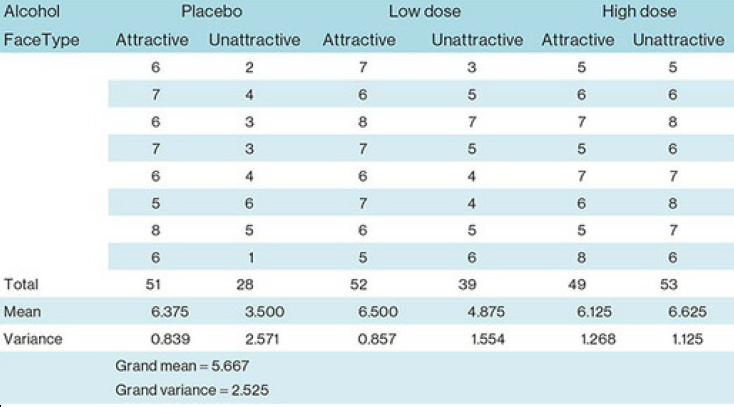
\includegraphics[width=1\textwidth,height=70mm]{Chapter 14 GLM 3 Factorial Designs/beergoggleeffect.PNG}
	\caption{Factorial design: 2 independent variable (Face type and dosage) }
\end{figure}


General Linear Model takes the form:
\begin{equation}
Y_i = b_0 + b_1X_{1i} + b_2X_{2i} + ...+ b_nX_{ni} + \varepsilon_i
\end{equation}

Just like the puppy therapy example, we can code participant's category membership on these variables with 0 and 1. 
However, in the alcohol and face attractiveness example, our linear equation we also need to consider about interaction effects. so the model will become:

\begin{equation}
\begin{split}
\text{Attractiveness}_i & = b_0 + b_1A_{i} + b_2B_{i} + b_3AB_{i} + \varepsilon_i \\
& = b_0 + b_1\text{FaceType}_{i} + b_2\text{Alcohol}_{i} + b_n\text{Interaction}_{i} + \varepsilon_i
\end{split}
\end{equation}

\begin{figure}[h]
	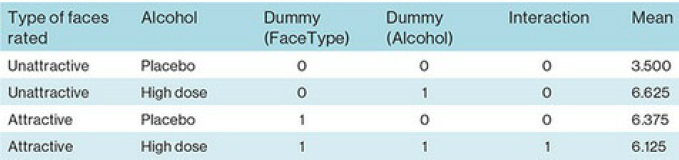
\includegraphics[width=1\textwidth,height=35mm]{Chapter 14 GLM 3 Factorial Designs/codingscheme.PNG}
	\caption{Coding scheme for the Linear Model}
\end{figure}

You code the interaction variable by multiplying the face dummy variable with the alcohol dummy variable. e.g. for someone receiving high dose of alcohol and rating unattractive faces, their dummy variables would be Facetype = 0, Alcohol = 0, Interaction = 0 x 0 = 0.

Similar to independent design,  $b_0$ represents \textbf{mean of the group for which all variables are coded as 0}, i.e. it is the mean value of the baseline category (in our example, it is the placebo group rating unattractive faces).
Similar to independent design, the predicted value of the outcome is our group mean.
\begin{equation}
\begin{split}
\text{Attractiveness}_i & = b_0 + b_1A_{i} + b_2B_{i} + b_3AB_{i} + \varepsilon_i \\
\bar{X}_{\text{unattractive, placebo}} & = b_0 + (b_1 \times 0) + (b_2 \times 0) + (b_3 \times 0) \\
b_0 & = \bar{X}_{\text{unattractive, placebo}} \\
& = 3.5
\end{split}
\end{equation}

For participants in placebo group rating attractive faces, $b_1$ represent difference between ratings of attractive and unattractive face in placebo condition. Or we can say it is the effect of type of face for baseline category of alcohol. It is model in the equation like this:
\begin{equation}
\begin{split}
\bar{X}_{\text{attractive, placebo}} & = b_0 + (b_1 \times 1) + (b_2 \times 0) + (b_3 \times 0) \\
& = b_0 + b_1 \\
& = \bar{X}_{\text{unattractive, placebo}} + b_1 \\
b_1 & = \bar{X}_{\text{attractive, placebo}} - \bar{X}_{\text{unattractive, placebo}} \\
& = 6.375 - 3.5\\
& = 2.875
\end{split}
\end{equation}
\clearpage

For participants in high dose of alcohol and rating unattractive faces. $b_2$ shows difference between ratings of unattractive faces after high alcohol dose. It is the effect of alcohol on baseline category type of face (i.e. Face type coded with 0). The model becomes:
\begin{equation}
\begin{split}
\bar{X}_{\text{unattractive, high dose}} & = b_0 + (b_1 \times 0) + (b_2 \times 1) + (b_3 \times 0) \\
& = b_0 + b_2 \\
& = \bar{X}_{\text{unattractive, placebo}} + b_2 \\
b_2 & = \bar{X}_{\text{unattractive, high dose}} - \bar{X}_{\text{unattractive, placebo}} \\
& = 6.625 - 3.5\\
& = 3.125
\end{split}
\end{equation}


For participants rating attractive faces after high dose of alcohol. We replace $b_0, b_1, b_2$ to get the equation:
\begin{equation}
\begin{split}
\bar{X}_{\text{attractive, high dose}} & = b_0 + (b_1 \times 1) + (b_2 \times 1) + (b_3 \times 1) \\
& = b_0 + b_1 + b_2 + b_3 \\
& = \bar{X}_{\text{unattractive, placebo}} + (\bar{X}_{\text{attractive, placebo}} - \bar{X}_{\text{unattractive, placebo}}) +  \\
 & (\bar{X}_{\text{unattractive, high dose}} - \bar{X}_{\text{unattractive, placebo}}) + b_3\\
b_3 & = \bar{X}_{\text{unattractive, placebo}} - \bar{X}_{\text{attractive, placebo}}  + \bar{X}_{\text{attractive, high dose}} - \bar{X}_{\text{unattractive, high dose}} \\
& = 3.5 - 6.375 + 6.125 - 6.625\\
& = -3.375
\end{split}
\end{equation}

$b_3$ compares the difference between ratings of unattractive and attractive faces in the placebo group to the same difference in the high dose group. More generally, it compares the effect of type of face after a placebo drink to the effect of type of face after a high dose of alcohol. 

If you rearrange the terms in the equation you can phrase the interaction in the opposite way: it represents effect of alcohol on ratings of attractiveness for attractive faces compared to unattractive ones.

Below is the plot of the interaction graph:
Difference between ratings of unattractive and attractive faces in the placebo group is 2.875. Difference between unattractive and attractive faces in high dose group is -0.500. If we plotted the difference values in the new graph, we will get the bottom left graph. The slope of the bottom left graph will be the value of $b_3$ (-.5 - -2.875 = -3.375)
\begin{figure}[h]
	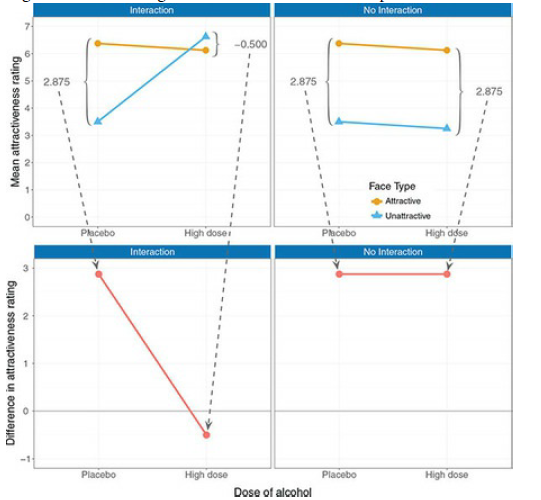
\includegraphics[width=1\textwidth,height=120mm]{Chapter 14 GLM 3 Factorial Designs/interactiongraph.PNG}
	\caption{Interaction graph that plot the 4 different means. Top left is the actual graph, top right is an example showing if there is no interaction effect (differences between attractiveness treatment group is the same)}
\end{figure}

\clearpage
\section{Behind the scenes of factorial designs}
Calculating F statistics for factorial design is similar in calculation as for independent design. Just that for $SS_M$ it is further subdivided to $SS_A$, $SS_B$ and $SS_{A\times B}$

\begin{figure}[ht]
	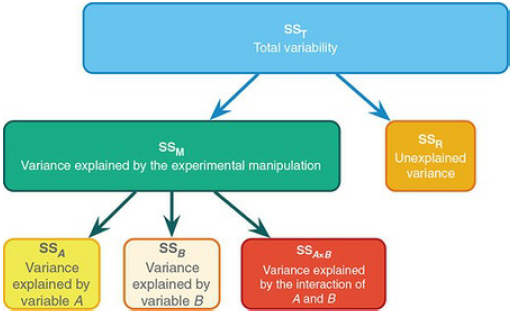
\includegraphics[width=1\textwidth,height=80mm]{Chapter 14 GLM 3 Factorial Designs/SSsubdivision.PNG}
	\caption{Breaking down the variance in a two-way factorial design}
\end{figure}

\section{Total of Squares, $SS_T$}

\begin{equation}
\begin{split}
\text{SS}_T & \sum^N_{i=1}(x_i - \bar{x}_{\text{grand}})^2\\
&= s^2_{grand}(N-1) 
\end{split}
\end{equation}

In our example then, $SS_T = 2.525(48 - 1) = 118.675$

\section{Model sum of squares, $SS_M$}
$SS_M$ in factorial design can be broken down to $SS_A$ and $SS_B$ and $SS_{A \times B}$. 
Recall $SS_M$ is the difference between what the model predicts and the overall mean of the variable outcome. We also seen that with predictors that represent group membership, what the model predicts is the group means. So We work out the model sum of squares by looking at the difference between each group mean and the overall mean. 

\begin{equation}
\text{SS}_M = \sum^k_{g=1} n_g(\bar{x}_g - \bar{x}_{grand})^2
\end{equation}

In our alcohol example, we have 6 separate groups for 2 IV. So, \\

 $SS_M = 8(6.375-5.667)^2 + 8(3.5-5.667)^2 + 8(6.5-5.667)^2 + 8(4.875-5.667)^2 + 8(6.125-5.667)^2 + 8(6.625-5.667)^2$ = 61.17

$df_M$ is $k-1$. So in this case $df$ = 5.

\section{Main effect for face type, $SS_A$}
To calculate $SS_A$, you group the scores into attractive and unattractive faces, regardless of alcohol dose. (i.e. group all the scores into 2 different groups). Then we apply the same equation for $SS_M$ to our data of 2 groups.

\begin{equation}
\text{SS}_A = \sum^k_{g=1} n_g(\bar{x}_g - \bar{x}_{grand})^2
\end{equation}

$\bar{x}_g$ is the group mean of either attractive and unattractive faces. $n_g$ is the number of scores in each group. i.e. number of people who rate unattractive and attractive. In our example, both groups have 24 participants.

$SS_{\text{facetype}} = 24(6.33-5.667)^2 + 24(5-5.667)^2$ \\

$df$ for $SS_A$ is k -1. So df is 1 in our example. 

\section{Main effect of alcohol, $SS_B$}
Similar to $SS_A$.
\begin{equation}
\text{SS}_B = \sum^k_{g=1} n_g(\bar{x}_g - \bar{x}_{grand})^2
\end{equation}

Alcohol split into 3 groups, no dose, low dose and high dose. \\
$SS_{\text{alcohol}} = 16(4.938-5.667)^2+ 16(5.668-5.667)^2 + 16(6.375-5.667)^2 = 16.53 $\\

Similarly, $df$ is k -1 . So in this example, $df$ = 2

\section{Interaction effect, $SS_{A \times B}$}
We can get the interaction effect by subtracting. 
\begin{equation}
SS_{A \times B} = SS_M - SS_A - SS_B
\end{equation}

In our example, it will be 61.17-21.32-16.53 = 23.32.

df can be calculated in 2 ways. Both will yield the same results:
\begin{enumerate}
\item $df_{A \times B} = df_M - df_A - df_B$
\item $df_{A \times B} = df_A \times df_B$
\end{enumerate}

\section{Residual sum of squares, $SS_R$}
$SS_R$ is calculated the same way. It represents error in the prediction from the model, but in experimental designs this also reflects individual differences in performance or variance that cannot be explained by factors that were systematically manipulated.

\begin{equation}
\begin{split}
SS_R & = \sum^k_{g=1} s^2_g (n_g - 1) \\
& = s^2_{group1}(n_1-1) + s^2_{group2}(n_2-1) + ... + s^2_{groupn}(n_n-1)
\end{split}
\end{equation}

$df_R = df_1 + df_2 + ... + df_n$

\section{F statistics}
\begin{equation}
\begin{split}
MS_A &= \frac{SS_A}{df_A}\\
MS_B &= \frac{SS_B}{df_B}\\
MS_{A \times B} &= \frac{SS_{A \times B}}{df_{A \times B}}\\
MS_R &= \frac{SS_R}{df_R}
\end{split}
\end{equation}

\begin{equation}
\begin{split}
F_A &= \frac{MS_A}{MS_R}\\
F_B &= \frac{MS_B}{MS_R}\\
F_{A \times B} &= \frac{MS_{A \times B}}{MS_R}\\
\end{split}
\end{equation}


\section{Model Assumptions in factorial designs}

All potential source of bias in The beast of bias applies. E.g. if you violated assumption of homogeneity of variance, you will use Welch procedure to correect. 

Pactical solution is to bootstrap post hoc tests so that these will be robusts.

